\subsection{Production and Mastering -- SDR On-Set and Digital Intermediate} \label{subsec:ff-onset-di-sdr}

	\subsubsection{Summary}
	The following section describes the ODTs to be used in standard dynamic range (SDR) feature film applications where images are viewed on-set, looks created, and transferred to post-production for final mastering on a standard dynamic range digital cinema projector.
	
	\subsubsection{Workflow}
	Figure \ref{fig:workflow1} shows a typical workflow for the creation and communication of looks during feature film production.  The complete workflow from camera to post is beyond the scope of this document. 
	
	\begin{figure*}[ht!]
	\centering
	    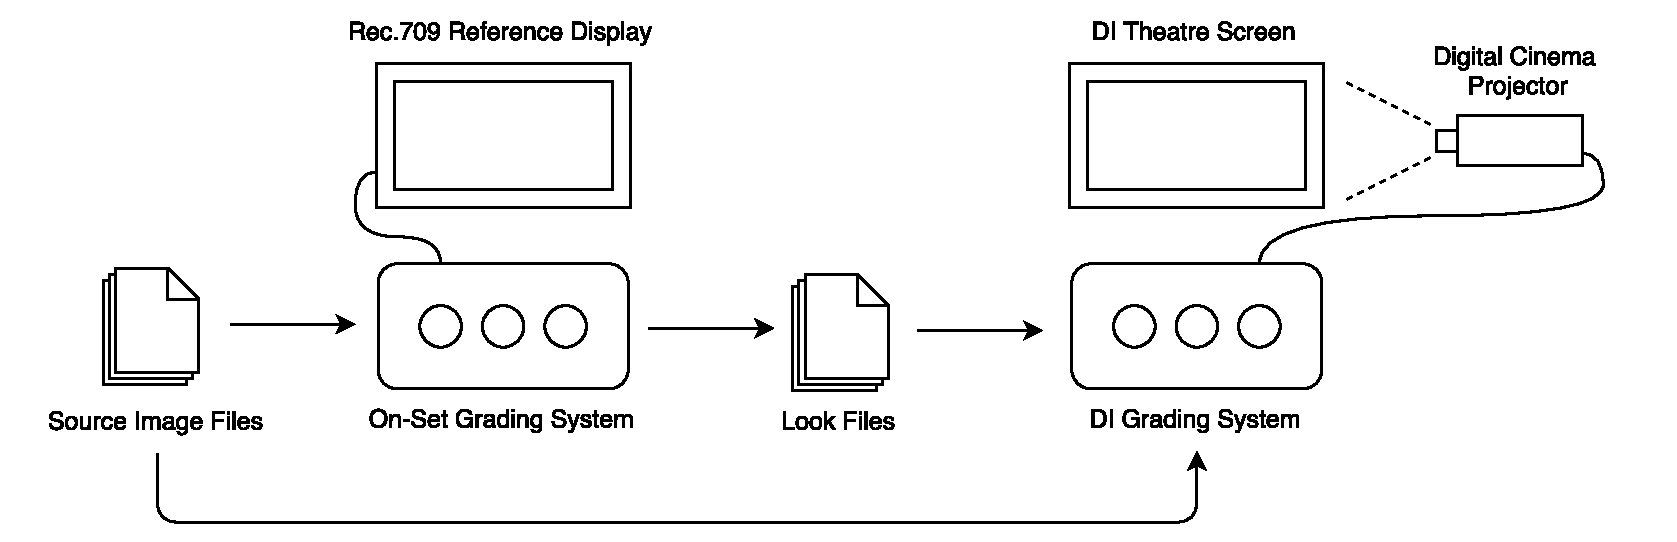
\includegraphics[width=4in]{images/workflows/workflow_ff-sdr-on-set-di.pdf}
	    \caption{\small Feature Film On-Set to SDR DI Workflow}
	    \label{fig:workflow1}
	\end{figure*}
	
	The workflow includes an on-set grading system with an attached SDR Rec.709 display and a DI color grading system with an attached SDR digital cinema projector.  Look files are created on-set using the on-set grading system and transferred to DI as a starting point for final color grading.
	
	Proper calibration an configuration of the displays is required.  Details of display configurations to be used are found in:
	
		\begin{itemize}
		  	\item DI grading system / SDR digital cinema projector -- \autoref{sec:odt-details-p3d60} - \nameref{sec:odt-details-p3d60}
  			\item On-set grading system / SDR Rec.709 display –- \autoref{sec:odt-details-rec709_d60sim} - \nameref{sec:odt-details-rec709_d60sim}
		\end{itemize}
		
	The recommended ODTs to be used with each of the systems and displays is listed in \autoref{tab:sum-ff-os-workflow}.
	
	\begin{table}[ht!]
	\centering
	\begin{tabular}{|p{0.5in}|p{1.2in}|p{3.75in}|}
	\hline
	\textbf{System}   & \textbf{Display}            & \textbf{Recommended ODT}                                                  \\ \hline
	On-set \newline Grading & Rec.709 Reference Monitor   & \texttt{\seqsplit{ODT.Academy.Rec709\_D60sim\_100nits\_dim.a1.0.3}} \\ \hline
	DI \newline Grading & P3 Digital Cinema Projector & \texttt{\seqsplit{ODT.Academy.P3D60\_48nits.a1.0.3}} \\ \hline
	\end{tabular}
	\caption[Workflows - Feature Film (Onset-DI) - Recommended ODTs]{Workflows - Feature Film (Onset-DI) - Recommended ODTs}
	\label{tab:sum-ff-os-workflow}
	\end{table}
	
	\subsubsection{Discussion}	
	Using the device configurations and ODTs described above will provide a colorimetric (i.e. measurement) match between the on-set and DI environments.  One should not assume that any given display matches either the specification, or other displays, used in the workflow without careful calibration.  Likewise, care should be taken to make sure the viewing environments match to insure a visual match.
	
	In the case that DI Grading digital cinema projector is not able to be configured according to the specifications in \autoref{sec:odt-details-p3d60} - \nameref{sec:odt-details-p3d60} the display may alternatively be configured according to the specifications in \autoref{sec:odt-details-p3dci} - \nameref{sec:odt-details-p3dci}.  In this case, the recommended ODT is \texttt{\seqsplit{ODT.Academy.P3DCI\_48nits.a1.0.3}}.